% Adjusting chapter title format for regular (numbered) chapters
\titleformat{\chapter}[display]
  {\normalfont\huge\bfseries\centering}{\chaptertitlename\ \thechapter}{20pt}{\Huge}

% Using similar styling for unnumbered chapters but without "Chapter" prefix
\titleformat{name=\chapter,numberless}
  {\normalfont\huge\bfseries\centering}{}{0pt}{\Huge}

\titlespacing*{\chapter}{0pt}{50pt}{40pt} % Adjust vertical spacing before and after the title

\chapter{Proposed Framework} % Ensures chapter numbering starts correctly
\label{chp:3}

% \section{Proposed Approach}

% This section introduces our comprehensive approach to evaluating AI system performance, summarized in Figure~\ref{fig:framework}. It takes as input the description of an AI system and a set of relevant specifications against which the AI system should be checked. The framework itself has four main components:

% \begin{enumerate}[\it (i)]
%     \item \emph{Sampling}: Choosing the original inputs for the AI system.
%     \item \emph{Testcase Generation}: Generating specific test cases from the sampled inputs according to the specifications.
%     \item \emph{Validation}: Checking the behavior of the AI system on the generated test cases, which can be fully-fledged \emph{verification} or more lightweight \emph{testing}.
%     \item \emph{Error Summarization}: Quantifying the performance of the AI system in terms of its global/local robustness/correctness.
% \end{enumerate}

% We focus on AI systems with DNN components performing classification tasks. We assume that an AI system $\S$ is a pair $(\F,\D)$ where:
% \begin{itemize}
%     \item $\F$ is the functional unit consisting of $n$ DNN \emph{classifiers} $f_1,\dots,f_n$ and a symbolic (software) component~$\omega$ such that given an input $\avec{x}=(x_1,\dots,x_n)$, the \emph{output}~$\F(\avec{x})$ is defined as $\omega(f_1(x_1),\dots,f_n(x_n))$.
%     \item $\D$ (for dataset) is a structure that describes valid inputs for each classifier $f_i$ and the corresponding correct outputs (i.e., labels). In particular, $\D.\mathit{next}_i(\mathit{param})$ returns a valid input $x_i$ for $f_i$, given the parameter $\mathit{param}$. Moreover, $\D.N_i$ is the number of distinct class labels for each classifier~$f_i$.
% \end{itemize}

% \begin{figure*}[h]
%   \centering
%   \begin{tikzpicture}[component/.style={fill=gray!80, text=white,
%       rounded corners, outer sep=1mm, text width=2.6cm, align=flush
%       center, minimum height=1.2cm, scale=0.8},
%     input/.style={draw, scale=0.8,  inner sep=2mm, outer sep=1mm}]\sf
    
%     \foreach \x/\al/\lab in {%
%       1/sampl/Sampling,%
%       2/gener/Testcase Generation,%
%       3/testing/Validation,%
%       4/summary/{Error\\ Summarisation}%
%     }{ \node[component] (\al) at (3.5*\x,0) {\textbf{\lab}}; }

%     \node[fit=(sampl)(summary), draw=gray, ultra thick] (approach) {};

%     \node[input] (aisystem) at (0.2, 0.5) {AI System $\S$};
%     \node[input] (spec)     at (0.2, -0.5) {Specifications $\Sigma$};

%     \foreach/\from/\to in {%
%       sampl/gener, gener/testing, testing/summary%
%     }{ \draw[-stealth, very thick] (\from) -- (\to); }

%     \draw[-latex, thick] (aisystem) -- (approach.179);
%     \draw[-latex, thick] (spec) -- (approach.181);
%   \end{tikzpicture}
%   \caption{Overview of the Proposed Framework}
%   \label{fig:framework}
% \end{figure*}

% \begin{example}
% \label{ex:mnist-adder}
% An instance of a simple AI system is an \emph{MNIST Digit Adder} $\S_{\text{MNIST}} = (\F,\D)$, where $\F = (\{f_{\text{mnist}}\}, +)$, $f_{\text{mnist}}$ is an MNIST Digit classifier and $\F$ takes as input two MNIST Digit images, recognizes the digits in the images, and computes their sum, i.e., $\F(x_1,x_2) = f_{\text{mnist}}(x_1) + f_{\text{mnist}}(x_2)$. $\D$ is the testing dataset for MNIST Digit consisting of 10,000 labeled images.
% \end{example}

% We assume that \emph{specifications} $\Sigma$ is a pair $(P, V)$, where $P$ is a set of perturbations against which we are characterizing the behavior of $\S$. Each perturbation comes with parameters to instantiate the set of all possible perturbations. $V$ is a validation flag, where if $V=t$, then we do testing, and if $V=v$, we do verification.

% \begin{example}
% To evaluate the correctness of the MNIST Digit Adder $\S_{\text{MNIST}}$, we define the specifications $\Sigma = (P, V)$ as follows: $P = \{\gaussian(0,0.1), \saltpepper(200:255, 0:5, 0.2), \rotation(3,30,3)\}$ and $V=t$. Here, $\gaussian(0,0.1)$ specifies Gaussian noise with a mean of $0$ and standard deviation of $0.1$, $\saltpepper(200:255,0:5,0.2)$ specifies salt and pepper noise, where 10\% of pixels are bleached up to values 200 to 255 and 10\% of pixels are darkened to values between 0 and 5, and $\rotation(3,30,3)$ specifies the set of rotations with the minimum rotation angle of 3, maximum of 30, and the step size of 3.
% \end{example}
% \section{Proposed Approach}

This chapter presents a comprehensive approach for AI systems, which may consist of one or multiple DNN components, each handling different tasks. Our framework addresses each DNN separately, recognizing that each has unique specifications, e.g., consider an AI system using the MNIST dataset for different purposes. One DNN might classify handwritten digits (0-9), while another might analyze pairs of digits to predict their sum or product. Although both DNNs work with digit images in this case, their properties in specifications differ due to their distinct tasks, even when using the same dataset. In other cases, such as an autonomous car, different DNNs might use different datasets designed for their specific tasks. One DNN might use labeled images for object detection (e.g., identifying pedestrians, vehicles, and road signs), while another DNN might use driving trajectories for path planning (e.g., predicting optimal routes). These diverse datasets ensure each DNN is tested according to its specific role within the AI system.

To address these diverse tasks and specifications, our framework comprises five components, summarized in Figure~\ref{fig:framework}.



\begin{enumerate}
  \item \emph{Specification}: defines key properties to guide testing. It includes details about the DNN architecture, environmental properties, and input data, like data type, sample size, and number of classes. This helps test the model thoroughly under different conditions.
    \item \emph{Sampling}: involves selecting a representative subset of inputs from a potentially vast input space. Depending on the testing objectives, this subset helps ensure that the tests are meaningful and cover various scenarios effectively.
    \item \emph{Testcase Generation}: applies the properties mentioned in the specifications to the sampled data to generate test cases.
    \item \emph{Testing Graph Analysis}: conducts both local and global coverage assessments. Locally, it focuses on an individual property to check its correctness. Globally, it examines multiple properties to understand their interdependencies and overall system behavior. By modeling these dependencies probabilistically, testing graph analysis provides a comprehensive view of AI system.
    \item \emph{Error Summarisation}: Quantifying the performance of the AI system by compiling and analyzing recorded errors. This analysis generates graphical reports and recommendations, helping to refine and improve the models.
\end{enumerate}

\begin{figure*}
  \centering
  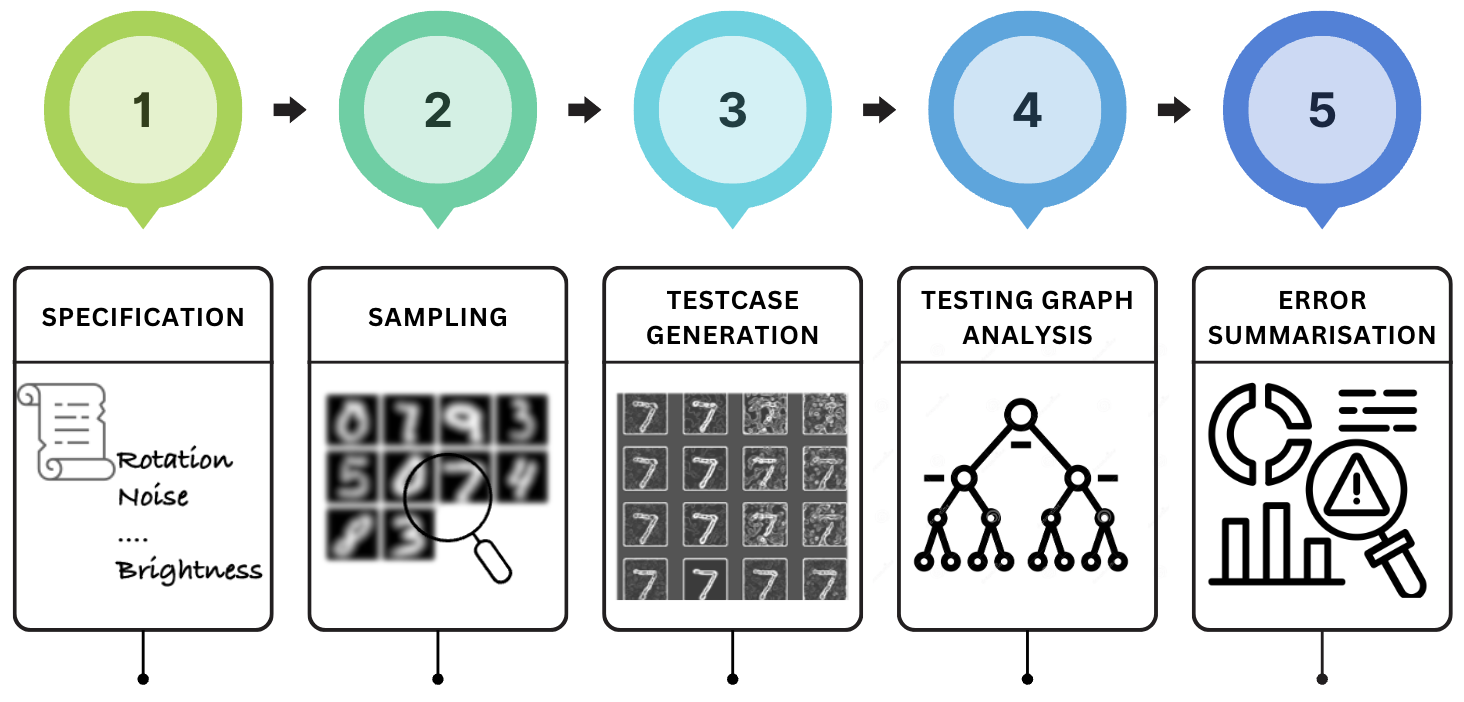
\includegraphics[width=\linewidth]{figures/fivesteps.png}
  \caption{Overview of the Proposed Framework}
  \label{fig:framework}
\end{figure*}
We focus on AI systems with DNN components performing various tasks, which may include classification, regression, clustering and more. Each DNN within the system has unique specifications. Formally, we define an AI system $ \mathcal{S} $ as follows:

 $\mathcal{F}$ is the functional unit comprises $ n $ DNN components $ f_1, \dots, f_n $, each handling different tasks, and a symbolic (software) component $ \omega $ that integrates the outputs of these DNNs. Given an input $ \vec{x} = (x_1, \dots, x_n) $, the output $ \mathcal{F}(\vec{x}) $ is defined as $ \omega(f_1(x_1), \dots, f_n(x_n)) $.

%  \begin{example}
%   \label{ex:mnist-adder}
%   An instance of a simple AI system is an \emph{MNIST Digit Adder} $\mathcal{S}_{\text{CNN}} = (\mathcal{F}, \mathcal{D})$, where $\mathcal{F} = (\{f_{\text{CNN}}\}, +)$. Here, $f_{\text{CNN}}$ is an MNIST digit classifier, and $\mathcal{F}$ takes as input two MNIST digit images, recognizes the digits in the images, and computes their sum. Specifically, $\mathcal{F}(x_1, x_2) = f_{\text{CNN}}(x_1) + f_{\text{CNN}}(x_2)$. The dataset $\mathcal{D} = \{ \mathcal{D}_{\text{mnist}} \}$ is the testing dataset for digits, consisting of 10,000 labeled images (0-9), where $\mathcal{D}_{\text{mnist}}$ is associated with the classifier $f_{\text{CNN}}$.
% \end{example}

\begin{example}
  \label{ex:mnist-adder}
  An instance of a simple AI system is an \emph{MNIST Digit Adder} $\mathcal{S} = (\mathcal{F})$. In this system, $\mathcal{F}$ consists of a DNN component $f_{\text{CNN}}$, which recognizes MNIST digits (0 to 9), and a software component $\omega$ that performs the addition.

  Formally, we define $\mathcal{F} = (\{f_{\text{CNN}}\}, \omega)$, where $\omega$ integrates the output of the DNN. The function $f_{\text{CNN}}$ takes single MNIST digit images as input and recognizes the digits. The software component $\omega$ can then pick any two recognized digits and compute their sum.

  For example, $\mathcal{F}$ can perform the task of digit addition:
  \begin{equation}
    \mathcal{F}(x_1, x_2) = \omega(f_{\text{CNN}}(x_1), f_{\text{CNN}}(x_2)),
  \end{equation}
  where $\omega(a, b) = a + b$.

  Given two MNIST digit images $x_1$ and $x_2$, $\mathcal{F}$ recognizes the digits and computes their sum.
\end{example}











% We focus on AI systems with DNN components performing classification tasks. We assume that an AI system $\S$ is a pair $(\F,\D)$ where:
% \begin{itemize}
%     \item $\F$ is the functional unit consisting of $n$ DNN \emph{classifiers} $f_1,\dots,f_n$ and a symbolic (software) component~$\omega$ such that given an input $\avec{x}=(x_1,\dots,x_n)$, the \emph{output}~$\F(\avec{x})$ is defined as $\omega(f_1(x_1),\dots,f_n(x_n))$.
%     \item \textcolor{blue}{ $\D$ (for dataset) is a structure that describes valid inputs and the corresponding correct outputs (i.e., labels). In particular, $\D.\mathit{next}(c)$ returns a valid input $\avec{x}$, given the parameter $c$, which represents the number of classes in the dataset. Moreover, $\D.N$ is the total number of distinct class labels.}
% \end{itemize}

\textcolor{blue}{
To ensure clarity in cases where multiple functional units are present, it is essential to specify which dataset belongs to which functional unit. Formally, let $\F = \{f_1, \dots, f_n\}$ represent the set of functional units and $\D = \{\D_1, \dots, \D_m\}$ represent the set of datasets. Each dataset $\D_j$ is associated with one or more functional units $\{f_{i_1}, \dots, f_{i_k}\} \subseteq \F$. This means that each $\D_j$ provides valid inputs and corresponding correct outputs specifically for the classifiers $f_{i_1}, \dots, f_{i_k}$. In this framework, each dataset $\D_j$ must clearly define its scope of association with the functional units. For instance, if $\D_1$ is associated with $f_1$ and $f_3$, then $\D_1$ provides valid inputs and correct outputs for both $f_1$ and $f_3$. This explicit association ensures that datasets are correctly utilized for their respective functional units, avoiding any ambiguity in the evaluation process.}


\textcolor{blue}{
To handle user-defined specifications and provide default behaviors when specifications are not explicitly defined, we assume that \emph{specifications} $\Sigma$ is a pair $(P, V)$, where $P$ is a set of perturbations against which we are characterizing the behavior of $\S$. Each perturbation comes with parameters to instantiate the set of all possible perturbations. $V$ is a validation flag, where if $V=t$, then we do testing, and if $V=v$, we do verification.}

\textcolor{blue}{If the user does not specify which classes to test or which properties to evaluate, our framework defaults to testing all classes in the dataset and evaluating all possible properties. Formally, let $\mathcal{C}$ be the set of all classes in the dataset $\D$ and $\mathcal{P}$ be the set of all possible properties. If the user does not define a subset $\mathcal{C}_u \subseteq \mathcal{C}$ or $\mathcal{P}_u \subseteq \mathcal{P}$, then $\mathcal{C}_u = \mathcal{C}$ and $\mathcal{P}_u = \mathcal{P}$, respectively.
}

% \begin{figure*}[h]
%   \centering
%   \begin{tikzpicture}[component/.style={fill=gray!80, text=white,
%       rounded corners, outer sep=1mm, text width=2.6cm, align=flush
%       center, minimum height=1.2cm, scale=0.8},
%     input/.style={draw, scale=0.8,  inner sep=2mm, outer sep=1mm}]\sf
    
%     \foreach \x/\al/\lab in {%
%       1/sampl/Sampling,%
%       2/gener/Testcase Generation,%
%       3/testing/Validation,%
%       4/summary/{Error\\ Summarisation}%
%     }{ \node[component] (\al) at (3.5*\x,0) {\textbf{\lab}}; }

%     \node[fit=(sampl)(summary), draw=gray, ultra thick] (approach) {};

%     \node[input] (aisystem) at (0.2, 0.5) {AI System $\S$};
%     \node[input] (spec)     at (0.2, -0.5) {Specifications $\Sigma$};

%     \foreach/\from/\to in {%
%       sampl/gener, gener/testing, testing/summary%
%     }{ \draw[-stealth, very thick] (\from) -- (\to); }

%     \draw[-latex, thick] (aisystem) -- (approach.179);
%     \draw[-latex, thick] (spec) -- (approach.181);
%   \end{tikzpicture}
%   \caption{Overview of the Proposed Framework}
%   \label{fig:framework}
% \end{figure*}



\begin{example}
  \label{ex:mnist-adder}
  An instance of a simple AI system is an \emph{MNIST Digit Adder} $\S_{\text{CNN}} = (\F,\D)$, where $\F = (\{f_{\text{CNN}}\}, +)$, $f_{\text{CNN}}$ is an MNIST Digit classifier and $\F$ takes as input two MNIST Digit images, recognizes the digits in the images, and computes their sum, i.e., $\F(x_1,x_2) = f_{\text{CNN}}(x_1) + f_{\text{CNN}}(x_2)$. $\D = \{ \D_{\text{mnist}} \}$ is the testing dataset for digits consisting of 10,000 labeled images (0-9), where $\D_{\text{mnist}}$ is associated with the classifier $f_{\text{CNN}}$.
  \end{example}
  
  We assume that \emph{specifications} $\Sigma$ is a pair $(P, V)$, where $P$ is a set of perturbations against which we are characterizing the behavior of $\S$. Each perturbation comes with parameters to instantiate the set of all possible perturbations. $V$ is a validation flag, where if $V=t$, then we do testing, and if $V=v$, we do verification.
  
  \begin{example}
  To evaluate the correctness of the  $\S_{\text{MNIST}}$, we define the specifications $\Sigma = (P, V)$ as follows: $P = \{\gaussian(0,0.1), \saltpepper(200:255, 0:5, 0.2), \rotation(3,30,3)\}$ and $V=t$. Here, $\gaussian(0,0.1)$ specifies Gaussian noise with a mean of $0$ and standard deviation of $0.1$, $\saltpepper(200:255,0:5,0.2)$ specifies salt and pepper noise, where 10\% of pixels are bleached up to values 200 to 255 and 10\% of pixels are darkened to values between 0 and 5, and $\rotation(3,30,3)$ specifies the set of rotations with the minimum rotation angle of 3, maximum of 30, and the step size of 3.
  \end{example}
  

\smallskip\noindent%
% Let's look into every component in detail.
% \section{Sampling}

% The sampling process involves a random but balanced choice of samples from each class, focusing exclusively on instances that the model has correctly predicted. Sampling happens independently for each classifier $f_i$. To ensure a representative and fair distribution of data across all classes, we sample the same number of instances from each class. The full sample $S_i$ for classifier $f_i$, $i=1,\dots,n$, is computed as:

% \begin{equation}
% S_i = \bigcup_{c=1}^{\D.N_i} S_i^c
% \end{equation}

% where $S_i^c$ is a subset of the correctly classified samples for a class $c$ consisting of $M_i$ (the number of samples for each class specific to $f_i$) elements:
% \[S_i^c = \big\{x = \D.next_i(class=c)\mid f_i(x)=c\big\}|_{M_i}\] 
% Note that each sample is obtained by a call to the method $\D.next_i$.

% \begin{example}
% Recall the MNIST Digit Adder system $\S_{\text{MNIST}}$ from Example~\ref{ex:mnist-adder}. When sampling, we make sure to select only correctly classified samples. For each digit $c$ (0 to 9), we randomly sample 100 images, i.e., $samp_1(\D,c,100)$ contains 100 inputs $x$ such that $f_{\text{CNN}}(x) = c$. In total, $S_1$ contains 1000 samples for all 10 classes.
% \end{example}

\section{Sampling}

The sampling process is designed to identify efficient and corner cases by employing a hybrid approach that combines Borderline-SMOTE and ADASYN. This combined method generates synthetic examples, enhancing class balance and model robustness. Borderline-SMOTE focuses on creating samples near decision boundaries, while ADASYN targets hard-to-learn examples, ensuring that both typical and challenging cases are effectively covered. It is important to note that this sampling process is used solely for testing purposes, not for training the model.

\textcolor{blue}{To ensure a balanced and representative dataset for testing, we perform the following steps for each classifier $f_i$ independently:}
\begin{itemize}
    % \item Randomly sample an equal number of correctly classified instances from each class.
    \item Apply Borderline-SMOTE to generate synthetic samples near decision boundaries to enhance class balance.
    \item Use ADASYN to adjust the number of synthetic samples for each minority class example based on its difficulty level.
\end{itemize}

The full sample $S_i$ for classifier $f_i$, $i=1,\dots,n$, is computed as:

\begin{equation}
S_i = \bigcup_{c=1}^{\D.N_i} S_i^c
\end{equation}

where $S_i^c$ is a subset of the correctly classified samples for a class $c$ consisting of $M_i$ (the number of samples for each class specific to $f_i$) elements:
\[S_i^c = \big\{x = \D.next_i(class=c)\mid f_i(x)=c\big\}|_{M_i}\]

\textcolor{blue}{After the initial sampling, we enhance $S_i^c$ by applying Borderline-SMOTE and ADASYN as follows:}
\[
S_i^c = S_i^c \cup \text{Borderline-SMOTE}(S_i^c) \cup \text{ADASYN}(S_i^c)
\]
Note that each sample is obtained by a call to the method $\D.next_i$.

% \begin{example}
% Recall the $\S_{\text{MNIST}}$ from Example~\ref{ex:mnist-adder}. When sampling, we make sure to select only correctly classified samples. For each digit $c$ (0 to 9), we randomly sample 100 images, i.e., $samp_1(\D,c,100)$ contains 100 inputs $x$ such that $f_{\text{CNN}}(x) = c$. After initial sampling, we apply Borderline-SMOTE to generate synthetic samples near the decision boundaries and ADASYN to further adjust the number of synthetic samples for challenging examples. In total, $S_1$ contains the original 1000 samples plus the additional synthetic samples for all 10 classes.
% \end{example}

\begin{tcolorbox}[colback=purple!2!white, colframe=purple, title=Challenges in Sampling]
  \begin{itemize}
    \item \textbf{Synthetic Sample Quality:} Ensuring generated samples represent true corner cases, not noise.
    \item \textbf{Computational Overhead:} Managing the intensive computation required for hybrid sampling.
    % \item \textbf{Parameter Tuning:} Finding optimal settings for Borderline-SMOTE and ADASYN to prevent ineffective sampling.
  \end{itemize}
  % \textbf{Mitigation Strategies:}
  % \begin{itemize}
  %   \item Use empirical evaluation to find optimal parameters for both techniques.
  %   \item Monitor the quality of synthetic samples to ensure they improve test coverage without adding noise.
  %   \item Limit the number of synthetic samples to balance computational efficiency and test coverage.
  % \end{itemize}
\end{tcolorbox}


\section{Test Case Generation}

The test case generation process aims to create test cases based on the given specifications to evaluate the correctness/robustness of the AI system.

Let $S_i^c$ be the set of samples produced in the sampling step for the classifier $f_i$ and a class $c$. For each perturbation $p\in P$, we generate a set $\T_p^c$ of test cases. Specifically, for each sample $x\in S$ we produce $testcases(p,c,x)$ according to $p$. Then $\T_p^c = \bigcup_{x\in S} testcases(p,c,x)$.

\begin{example}
To generate test cases for the MNIST Digit Adder $\S_{\text{MNIST}}$, we use the specifications defined in Example 2, which include noise and rotation perturbations. Let $S$ be the set of sampled images obtained in Example 3. For each pair of images $(x_1, x_2) \in S$, we define the following test cases:
\begin{itemize}
    \item \textbf{Rotation}: For a given angle $\theta$, generate the perturbed images $x_1' = \text{rotate}(x_1, \theta)$ and $x_2' = \text{rotate}(x_2, \theta)$. The test case is then:
    $\mathcal{T}_{\text{rotation}} = \left\{(x_1', x_2') \mid x_1', x_2' \in \text{rotate}(S, \theta)\right\}$
    \item \textbf{Noise}: For a given mean $\mu$ and standard deviation $\sigma$, generate the perturbed images $x_1'' = \text{noise}(x_1, \mu, \sigma)$ and $x_2'' = \text{noise}(x_2, \mu, \sigma)$. The test case is then:
    $\mathcal{T}_{\text{noise}} = \left\{(x_1'', x_2'') \mid x_1'', x_2'' \in \text{noise}(S, \mu, \sigma)\right\}$
\end{itemize}
The overall set of test cases $\mathcal{T}$ is the union of the individual test cases:
$\mathcal{T} = \mathcal{T}_{\text{rotation}} \cup \mathcal{T}_{\text{noise}}$
\end{example}

\section{Validation}

The validation process aims to evaluate the correctness and robustness of the AI system under various perturbations.

Fix a perturbation \( p \in P \) and a class \( c \). For every test case in \( \mathcal{T}_p^c \), we store the results in the form:
\[ \text{Raw}_{p, c} = \Big\{\big(\text{query}(f_i, x, c), f_i(x)_c\big) \mid x \in \mathcal{T}_p^c \Big\} \]

After generating test cases, measure the AI subsystem's confidence for each class under each type of property.

\subsection{Local Robustness}

Local robustness involves evaluating the AI subsystem's performance on individual images subjected to various transformations. For each image \( x \) from a set of samples \( S_i^c \), the AI subsystem produces a confidence score \( f_i(x) \) representing its certainty in recognizing the class \( c \). The local robustness for a transformation \( T \) applied to an image \( x \) is defined as:

\[ \text{Local Robustness}(x, T) = f_i(T(x)) \]

where \( T \) can be any transformation such as noise addition, rotation, brightness adjustment, occlusion, or scaling. Each transformation is evaluated to determine its impact on the confidence score.

To quantify local robustness, we compute the accuracy for each transformation applied to the images of a specific class:

\[
\text{Local Robustness}(c, T) = \frac{1}{|S_i^c|} \sum_{x \in S_i^c} \mathbb{I}[f_i(T(x)) = c]
\]

where:
- \(\text{Local Robustness}(c, T)\) is the accuracy of the classifier \( f_i \) for class \( c \) under transformation \( T \).
- \( \mathbb{I}[f_i(T(x)) = c] \) is an indicator function that is 1 if the classifier correctly predicts the class \( c \) for the transformed image \( T(x) \), and 0 otherwise.
- \(|S_i^c|\) is the number of correctly classified images in class \( c \).

\begin{example}
Consider the class \( c = 3 \) and the transformation \( T \) being a rotation by 25 degrees. If we have three images \( x_1, x_2, x_3 \) from class \( c \), and the model correctly classifies \( x_1 \) and \( x_2 \) but misclassifies \( x_3 \), the local robustness is computed as follows:

\[
\text{Local Robustness}(3, \text{rotation}) = \frac{1}{3} (\mathbb{I}[f_i(\text{rotate}(x_1, 25)) = 3] + 
\]
\[
\mathbb{I}[f_i(\text{rotate}(x_2, 25)) = 3] + \mathbb{I}[f_i(\text{rotate}(x_3, 25)) = 3])
\]


If the indicator values are 1, 1, and 0 respectively, the local robustness would be:

\[
\text{Local Robustness}(3, \text{rotation}) = \frac{1}{3} (1 + 1 + 0) = \frac{2}{3} \approx 0.67
\]
\end{example}

\subsection{Global Robustness}

Global robustness evaluates the AI subsystem's performance across multiple images and transformations. It is an aggregate measure of how well the AI system performs under various properties on a set of images $S_i^c$.

For a given transformation $T$ and a set of images $S_i^c$, the global robustness is defined as:

$$ \text{Global Robustness}(S_i^c, T) = \frac{1}{|S_i^c|} \sum_{x \in S_i^c} \mathbb{I}[f_i(T(x)) = c] $$

This measures the average confidence score for the AI subsystem over the entire dataset when subjected to a particular transformation.

To quantify global robustness, we compute the expected confidence score over all transformations and images. Depending on whether the relationship is AND or OR, the formulas vary:

\textbf{AND Relationship:}

For an AND relationship between transformations, the global robustness is calculated as:

$$ P(\text{Property 1} \cap \text{Property 2}) = P(\text{Property 1}) \times P(\text{Property 2}) $$

\textbf{OR Relationship:}

For an OR relationship between transformations, the global robustness is calculated as:

$$ P(\text{Property 1} \cup \text{Property 2}) = P(\text{Property 1}) + P(\text{Property 2}) - P(\text{Property 1} \cap \text{Property 2}) $$

\begin{example}
Consider a pair of images $(x_1, x_2)$ representing the digits '3' and '5'. Let the transformation $T$ be rotation. If the model's confidence scores for these transformations are as follows:

$$
\begin{aligned}
&f_i(\text{rotation}(x_1)) = 0.78, \\
&f_i(\text{rotation}(x_2)) = 0.85,
\end{aligned}
$$

For the AND relationship, the global correctness for the pair is computed as follows:

$$P(\text{Global Robustness}_{\text{AND}}) = 0.78 \times 0.85$$

For the OR relationship, the global correctness for the pair is computed as follows:

$$P(\text{Global Robustness}_{\text{OR}}) = 0.78 + 0.85 - (0.78 \times 0.85)$$

(Note: The complete OR relationship formula requires including all images and transformations as per the OR formula.)

\end{example}

\subsection{Use Cases and Examples}
To illustrate the application of ProbLog for global robustness in real-world scenarios, we present the following use cases:

\subsubsection{Use Case 1: Handwritten Digit Recognition}
\textbf{Scenario:} Consider an AI system designed to recognize handwritten digits, such as the MNIST dataset. The system is evaluated under various transformations, including noise addition, rotation, and brightness adjustment. The goal is to determine the global robustness of the system in recognizing digit pairs correctly under these properties.

The tables below provide the probabilities for correctly recognizing digit pairs under different conditions (AND and OR relationships) for an MNIST 2-digit addition system. Each world represents a different combination of transformations applied to the digits.

\begin{table}[h]
    \centering
    \caption{Specification Probabilities for MNIST 2-Digit Addition Under Different Transformations}
    \label{tab:mnist_prob_and_or}
    \resizebox{\textwidth}{!}{%
    \begin{tabular}{|c|c|c|c|c|c|}
    \hline
    \textbf{World} & \textbf{Conditions} & \textbf{Probability Expression (AND)} & \textbf{Probability (AND)} & \textbf{Probability Expression (OR)} & \textbf{Probability (OR)} \\
    \hline
    $w_1$ & \{noise(0), noise(1)\} & $0.85 \cdot 0.8$ & $0.68$ & $0.85 + 0.8 - (0.85 \cdot 0.8)$ & $0.97$ \\
    $w_2$ & \{noise(0), correct(1)\} & $0.85 \cdot 0.9$ & $0.765$ & $0.85 + 0.9 - (0.85 \cdot 0.9)$ & $0.985$ \\
    $w_3$ & \{correct(0), noise(1)\} & $0.9 \cdot 0.8$ & $0.72$ & $0.9 + 0.8 - (0.9 \cdot 0.8)$ & $0.98$ \\
    $w_4$ & \{rotation(0), correct(1)\} & $0.88 \cdot 0.9$ & $0.792$ & $0.88 + 0.9 - (0.88 \cdot 0.9)$ & $0.992$ \\
    $w_5$ & \{correct(0), rotation(1)\} & $0.9 \cdot 0.77$ & $0.693$ & $0.9 + 0.77 - (0.9 \cdot 0.77)$ & $0.977$ \\
    $w_6$ & \{rotation(0), rotation(1)\} & $0.88 \cdot 0.77$ & $0.6776$ & $0.88 + 0.77 - (0.88 \cdot 0.77)$ & $0.9696$ \\
    $w_7$ & \{noise(0), rotation(1)\} & $0.85 \cdot 0.77$ & $0.6545$ & $0.85 + 0.77 - (0.85 \cdot 0.77)$ & $0.9655$ \\
    $w_8$ & \{rotation(0), noise(1)\} & $0.88 \cdot 0.8$ & $0.704$ & $0.88 + 0.8 - (0.88 \cdot 0.8)$ & $0.976$ \\
    $w_9$ & \{correct(0), correct(1)\} & $0.9 \cdot 0.9$ & $0.81$ & $0.9 + 0.9 - (0.9 \cdot 0.9)$ & $0.99$ \\
    \hline
    \end{tabular}
    }
\end{table}

\textbf{Explanation:} The table shows the global correctness probabilities for pairs of digits under various transformation conditions. Each row represents a different combination of transformations applied to the two digits in the pair:
- AND Probability: The probability that both digits are correctly recognized under the specified transformations.
- OR Probability: The probability that at least one of the digits is correctly recognized under the specified transformations.

For example, in world $w_1$, both digits are subjected to noise, leading to an AND probability of $0.68$ and an OR probability of $0.97$.

\textbf{Problog Code:}
\begin{mdframed}[leftline=false, rightline=false, topline=true, bottomline=true]
\scriptsize
\begin{verbatim}
% Define probabilities for digit 0 under different transformations
0.9::noise_0. % Digit 0 correctly predicted with 90% probability under noise
0.85::brightness_0. % Digit 0 correctly predicted with 85% probability under brightness
0.88::rotation_0. % Digit 0 correctly predicted with 88% probability under rotation

% Define probabilities for digit 1 under different transformations
0.8::noise_1. % Digit 1 correctly predicted with 80% probability under noise
0.75::brightness_1. % Digit 1 correctly predicted with 75% probability under brightness
0.77::rotation_1. % Digit 1 correctly predicted with 77% probability under rotation

% Define rules for correct prediction under each transformation for digit 0
correct_noise_0 :- noise_0.
correct_brightness_0 :- brightness_0.
correct_rotation_0 :- rotation_0.

% Define rules for correct prediction under each transformation for digit 1
correct_noise_1 :- noise_1.
correct_brightness_1 :- brightness_1.
correct_rotation_1 :- rotation_1.

% Define rules for incorrect prediction under each transformation for digit 0
wrong_noise_0 :- +correct_noise_0.
wrong_brightness_0 :- +correct_brightness_0.
wrong_rotation_0 :- +correct_rotation_0.

% Define rules for incorrect prediction under each transformation for digit 1
wrong_noise_1 :- +correct_noise_1.
wrong_brightness_1 :- +correct_brightness_1.
wrong_rotation_1 :- +correct_rotation_1.

% Define rules for correct prediction of both digits under noise
pair_correct_noise_0_1 :- correct_noise_0, correct_noise_1.
% Define rules for incorrect prediction of both digits under noise
pair_wrong_noise_0_1 :- wrong_noise_0, wrong_noise_1.

% Define global correctness based on either both correct or both incorrect under noise
global_correct_noise_0_1 :- pair_correct_noise_0_1; pair_wrong_noise_0_1.

% Query the global correctness under noise
query(global_correct_noise_0_1).
\end{verbatim}
\end{mdframed}
\captionof{figure}{Problog code snippet for evaluating handwritten digit recognition under noise, brightness, and rotation transformations.}

\textbf{Explanation:} In this scenario, we are interested in the global correctness of recognizing pairs of digits (0 and 1) under different transformations. The ProbLog code models the local robustness probabilities for each transformation and combines them to evaluate the global correctness.

\subsubsection{Use Case 2: Autonomous Vehicle Perception}

\textbf{Scenario:} An AI system used in autonomous vehicles must reliably detect objects such as vehicles under various weather conditions (rain, sand, fog, and snow). The goal is to evaluate the system's robustness in identifying these objects correctly under these weather conditions.

\begin{mdframed}[leftline=false, rightline=false, topline=true, bottomline=true]
  \scriptsize
  \begin{verbatim}

% Probabilities for Vehicle Detection under Different Weather Conditions
0.75::rain_vehicle. % Vehicle correctly detected with 75% probability under rain
0.55::fog_vehicle. % Vehicle correctly detected with 55% probability under fog
0.7::snow_vehicle. % Vehicle correctly detected with 70% probability under snow

% Correct Detection Rules for Vehicle
correct_rain_vehicle :- rain_vehicle.
correct_fog_vehicle :- fog_vehicle.
correct_snow_vehicle :- snow_vehicle.

% Incorrect Detection Rules for Vehicle
wrong_rain_vehicle :- +correct_rain_vehicle.
wrong_fog_vehicle :- +correct_fog_vehicle.
wrong_snow_vehicle :- +correct_snow_vehicle.

% AND conditions for Vehicle Detection under all weather conditions
global_correct_vehicle_and :- correct_rain_vehicle, correct_fog_vehicle, correct_snow_vehicle.

% OR conditions for Vehicle Detection under any weather condition
global_correct_vehicle_or :- correct_rain_vehicle; correct_fog_vehicle; correct_snow_vehicle.

% Mixed conditions (AND & OR) for Vehicle Detection
global_correct_mixed_vehicle :- correct_rain_vehicle, (correct_fog_vehicle; correct_snow_vehicle).

% Queries for Global Correctness
query(global_correct_vehicle_and).
query(global_correct_vehicle_or).
query(global_correct_mixed_vehicle).
\end{verbatim}
\end{mdframed}
\captionof{figure}{Problog code snippet for evaluating vehicle detection under different weather conditions.}

\textbf{Explanation:} The ProbLog code assesses the global robustness of the AI system in detecting objects (vehicles) under individual and combined weather conditions. This ensures that the system can reliably perform in diverse environmental scenarios.

\begin{table}[h]
  \centering
  \caption{Specification Probabilities (AND) for Vehicle Detection Under Different Weather Conditions \\
  \( P(A \cap B \cap C) = P(A) \times P(B) \times P(C) \)}
  \label{tab:veh_prob_and}
  \resizebox{\textwidth}{!}{%
  \begin{tabular}{|c|c|c|c|}
  \hline
  \textbf{World} & \textbf{Conditions} & \textbf{Probability Expression (AND)} & \textbf{Probability (AND)} \\
  \hline
  $w_1$ & \{rain, fog\} & $0.75 \times 0.55$ & $0.4125$ \\
  $w_2$ & \{rain, snow\} & $0.75 \times 0.7$ & $0.525$ \\
  $w_3$ & \{rain, sand\} & $0.75 \times 0.6$ & $0.45$ \\
  $w_4$ & \{fog, snow\} & $0.55 \times 0.7$ & $0.385$ \\
  $w_5$ & \{fog, sand\} & $0.55 \times 0.6$ & $0.33$ \\
  $w_6$ & \{snow, sand\} & $0.7 \times 0.6$ & $0.42$ \\
  $w_7$ & \{rain, fog, snow\} & $0.75 \times 0.55 \times 0.7$ & $0.28875$ \\
  $w_8$ & \{rain, fog, sand\} & $0.75 \times 0.55 \times 0.6$ & $0.2475$ \\
  $w_9$ & \{rain, snow, sand\} & $0.75 \times 0.7 \times 0.6$ & $0.315$ \\
  $w_{10}$ & \{fog, snow, sand\} & $0.55 \times 0.7 \times 0.6$ & $0.231$ \\
  \hline
  \end{tabular}
  }
\end{table}

\textbf{Explanation:} This table shows the global correctness probabilities for detecting vehicles under different combinations of weather conditions using AND relationships. Each row represents a different combination of weather conditions applied to the detection scenario:
- AND Probability: The probability that the vehicle is correctly detected under all specified weather conditions.

For example, in world $w_1$, the vehicle detection system is subjected to rain and fog, leading to an AND probability of $0.4125$.

\begin{table}[h]
  \centering
  \caption{Specification Probabilities (OR) for Vehicle Detection Under Different Weather Conditions \\
  \( P(A \cup B \cup C) = P(A) + P(B) + P(C) - P(A \cap B) - P(A \cap C) - P(B \cap C) + P(A \cap B \cap C) \)}
  \label{tab:veh_prob_or}
  \resizebox{\textwidth}{!}{%
  \begin{tabular}{|c|c|c|c|}
  \hline
  \textbf{World} & \textbf{Conditions} & \textbf{Probability Expression (OR)} & \textbf{Probability (OR)} \\
  \hline
  $w_1$ & \{rain; fog\} & $0.75 + 0.55 - (0.75 \times 0.55)$ & $0.8875$ \\
  $w_2$ & \{rain; snow\} & $0.75 + 0.7 - (0.75 \times 0.7)$ & $0.925$ \\
  $w_3$ & \{rain; sand\} & $0.75 + 0.6 - (0.75 \times 0.6)$ & $0.9$ \\
  $w_4$ & \{fog; snow\} & $0.55 + 0.7 - (0.55 \times 0.7)$ & $0.835$ \\
  $w_5$ & \{fog; sand\} & $0.55 + 0.6 - (0.55 \times 0.6)$ & $0.82$ \\
  $w_6$ & \{snow; sand\} & $0.7 + 0.6 - (0.7 \times 0.6)$ & $0.88$ \\
  $w_7$ & \{rain; fog; snow\} & $0.75 + 0.55 + 0.7 - (0.75 \times 0.55) - (0.75 \times 0.7) - (0.55 \times 0.7) + (0.75 \times 0.55 \times 0.7)$ & $0.966625$ \\
  $w_8$ & \{rain; fog; sand\} & $0.75 + 0.55 + 0.6 - (0.75 \times 0.55) - (0.75 \times 0.6) - (0.55 \times 0.6) + (0.75 \times 0.55 \times 0.6)$ & $0.95125$ \\
  $w_9$ & \{rain; snow; sand\} & $0.75 + 0.7 + 0.6 - (0.75 \times 0.7) - (0.75 \times 0.6) - (0.7 \times 0.6) + (0.75 \times 0.7 \times 0.6)$ & $0.967$ \\
  $w_{10}$ & \{fog; snow; sand\} & $0.55 + 0.7 + 0.6 - (0.55 \times 0.7) - (0.55 \times 0.6) - (0.7 \times 0.6) + (0.55 \times 0.7 \times 0.6)$ & $0.938$ \\
  \hline
  \end{tabular}
  }
\end{table}

\textbf{Explanation:} This table shows the global correctness probabilities for detecting vehicles under different combinations of weather conditions using OR relationships. Each row represents a different combination of weather conditions applied to the detection scenario:
- OR Probability: The probability that the vehicle is correctly detected under at least one of the specified weather conditions.

For example, in world $w_1$, the vehicle detection system is subjected to rain and fog, leading to an OR probability of $0.8875$.




% \subsection{Use Cases and Examples}

% To illustrate the application of Problog for global robustness in real-world scenarios, we present the following use cases:

% \subsection{Use Case 1: Handwritten Digit Recognition}

% \textbf{Scenario:} Consider an AI system designed to recognize handwritten digits, such as the MNIST dataset. The system is evaluated under various transformations, including noise addition, rotation, and brightness adjustment. The goal is to determine the global robustness of the system in recognizing digit pairs correctly under these properties.


  
%   \begin{table}[h]
%     \centering
  
%     \caption{Specification Probabilities for MNIST 2-Digit Addition Under Different Transformations}
%     \label{tab:mnist_prob_and_or}
  
%     \resizebox{\textwidth}{!}{%
%     \begin{tabular}{|c|c|c|c|c|c|}
%     \hline
%     \textbf{World} & \textbf{Conditions} & \textbf{Probability Expression (AND)} & \textbf{Probability (AND)} & \textbf{Probability Expression (OR)} & \textbf{Probability (OR)} \\
%     \hline
%     $w_1$ & \{noise(0), noise(1)\} & $0.85 \cdot 0.8$ & $0.68$ & $0.85 + 0.8 - (0.85 \cdot 0.8)$ & $0.97$ \\
%     $w_2$ & \{noise(0), correct(1)\} & $0.85 \cdot 0.9$ & $0.765$ & $0.85 + 0.9 - (0.85 \cdot 0.9)$ & $0.985$ \\
%     $w_3$ & \{correct(0), noise(1)\} & $0.9 \cdot 0.8$ & $0.72$ & $0.9 + 0.8 - (0.9 \cdot 0.8)$ & $0.98$ \\
%     $w_4$ & \{rotation(0), correct(1)\} & $0.88 \cdot 0.9$ & $0.792$ & $0.88 + 0.9 - (0.88 \cdot 0.9)$ & $0.992$ \\
%     $w_5$ & \{correct(0), rotation(1)\} & $0.9 \cdot 0.77$ & $0.693$ & $0.9 + 0.77 - (0.9 \cdot 0.77)$ & $0.977$ \\
%     $w_6$ & \{rotation(0), rotation(1)\} & $0.88 \cdot 0.77$ & $0.6776$ & $0.88 + 0.77 - (0.88 \cdot 0.77)$ & $0.9696$ \\
%     $w_7$ & \{noise(0), rotation(1)\} & $0.85 \cdot 0.77$ & $0.6545$ & $0.85 + 0.77 - (0.85 \cdot 0.77)$ & $0.9655$ \\
%     $w_8$ & \{rotation(0), noise(1)\} & $0.88 \cdot 0.8$ & $0.704$ & $0.88 + 0.8 - (0.88 \cdot 0.8)$ & $0.976$ \\
%     $w_9$ & \{correct(0), correct(1)\} & $0.9 \cdot 0.9$ & $0.81$ & $0.9 + 0.9 - (0.9 \cdot 0.9)$ & $0.99$ \\
%     \hline
%     \end{tabular}
%     }
%     \end{table}
  



% \textbf{Problog Code:}
% \begin{mdframed}[leftline=false, rightline=false, topline=true, bottomline=true]
% \scriptsize
% \begin{verbatim}
% % Define probabilities for digit 0 under different transformations
% 0.9::noise_0. % Digit 0 correctly predicted with 90% probability under noise
% 0.85::brightness_0. % Digit 0 correctly predicted with 85% probability under brightness
% 0.88::rotation_0. % Digit 0 correctly predicted with 88% probability under rotation

% % Define probabilities for digit 1 under different transformations
% 0.8::noise_1. % Digit 1 correctly predicted with 80% probability under noise
% 0.75::brightness_1. % Digit 1 correctly predicted with 75% probability under brightness
% 0.77::rotation_1. % Digit 1 correctly predicted with 77% probability under rotation

% % Define rules for correct prediction under each transformation for digit 0
% correct_noise_0 :- noise_0.
% correct_brightness_0 :- brightness_0.
% correct_rotation_0 :- rotation_0.

% % Define rules for correct prediction under each transformation for digit 1
% correct_noise_1 :- noise_1.
% correct_brightness_1 :- brightness_1.
% correct_rotation_1 :- rotation_1.

% % Define rules for incorrect prediction under each transformation for digit 0
% wrong_noise_0 :- +correct_noise_0.
% wrong_brightness_0 :- +correct_brightness_0.
% wrong_rotation_0 :- +correct_rotation_0.

% % Define rules for incorrect prediction under each transformation for digit 1
% wrong_noise_1 :- +correct_noise_1.
% wrong_brightness_1 :- +correct_brightness_1.
% wrong_rotation_1 :- +correct_rotation_1.

% % Define rules for correct prediction of both digits under noise
% pair_correct_noise_0_1 :- correct_noise_0, correct_noise_1.
% % Define rules for incorrect prediction of both digits under noise
% pair_wrong_noise_0_1 :- wrong_noise_0, wrong_noise_1.

% % Define global correctness based on either both correct or both incorrect under noise
% global_correct_noise_0_1 :- pair_correct_noise_0_1; pair_wrong_noise_0_1.

% % Query the global correctness under noise
% query(global_correct_noise_0_1).
% \end{verbatim}
% \end{mdframed}
% \captionof{figure}{Problog code snippet for evaluating handwritten digit recognition under noise, brightness, and rotation transformations.}



% \textbf{Explanation:} In this scenario, we are interested in the global correctness of recognizing pairs of digits (0 and 1) under different transformations. The Problog code models the local robustness probabilities for each transformation and combines them to evaluate the global correctness.


%   \subsection{Use Case 2: Autonomous Vehicle Perception}

% \textbf{Scenario:} An AI system used in autonomous vehicles must reliably detect objects such as pedestrians and vehicles under various weather conditions (rain, fog, and snow). The goal is to evaluate the system's robustness in identifying these objects correctly under these weather conditions.



% \begin{mdframed}[leftline=false, rightline=false, topline=true, bottomline=true]
%   \scriptsize
%   \begin{verbatim}

%   % Probabilities for Vehicle Detection under Different Weather Conditions
%   0.75::rain_vehicle. % Vehicle correctly detected with 75% probability under rain
%   0.55::fog_vehicle. % Vehicle correctly detected with 55% probability under fog
%   0.7::snow_vehicle. % Vehicle correctly detected with 70% probability under snow

  
%   % Correct Detection Rules for Vehicle
%   correct_rain_vehicle :- rain_vehicle.
%   correct_fog_vehicle :- fog_vehicle.
%   correct_snow_vehicle :- snow_vehicle.
  
%   % Incorrect Detection Rules for Vehicle
%   wrong_rain_vehicle :- +correct_rain_vehicle.
%   wrong_fog_vehicle :- +correct_fog_vehicle.
%   wrong_snow_vehicle :- +correct_snow_vehicle.
  

%   % AND conditions for Vehicle Detection under all weather conditions
%   global_correct_vehicle_and :- correct_rain_vehicle, correct_fog_vehicle, correct_snow_vehicle.
  
%   % OR conditions for Vehicle Detection under any weather condition
%   global_correct_vehicle_or :- correct_rain_vehicle; correct_fog_vehicle; correct_snow_vehicle.
  
%   % Mixed conditions (AND & OR) for Vehicle Detection
%   global_correct_mixed_vehicle :- correct_rain_vehicle, (correct_fog_vehicle; correct_snow_vehicle).
  
%   % Queries for Global Correctness

%   query(global_correct_vehicle_and).
%   query(global_correct_vehicle_or).
%   query(global_correct_mixed_vehicle).
%   \end{verbatim}
%   \end{mdframed}
%   \captionof{figure}{Problog code snippet for evaluating  vehicle detection under different weather conditions.}
  
  

% \textbf{Explanation:} he Problog code assesses the global robustness of the AI system in detecting objects (pedestrians and vehicles) under individual and combined weather conditions. This ensures that the system can reliably perform in diverse environmental scenarios.

% \begin{table}[h]
%   \centering
%   \caption{Specification Probabilities (AND) for Vehicle Detection Under Different Weather Conditions \\
%   \( P(A \cap B \cap C) = P(A) \times P(B) \times P(C) \)}
%   \label{tab:veh_prob_and}
%   \resizebox{\textwidth}{!}{%
%   \begin{tabular}{|c|c|c|c|}
%   \hline
% \textbf{World} & \textbf{Conditions} & \textbf{Probability Expression (AND)} & \textbf{Probability (AND)} \\
%   \hline
%   $w_1$ & \{rain, fog\} & $0.75 \times 0.55$ & $0.4125$ \\
%   $w_2$ & \{rain, snow\} & $0.75 \times 0.7$ & $0.525$ \\
%   $w_3$ & \{rain, sand\} & $0.75 \times 0.6$ & $0.45$ \\
%   $w_4$ & \{fog, snow\} & $0.55 \times 0.7$ & $0.385$ \\
%   $w_5$ & \{fog, sand\} & $0.55 \times 0.6$ & $0.33$ \\
%   $w_6$ & \{snow, sand\} & $0.7 \times 0.6$ & $0.42$ \\
%   $w_7$ & \{rain, fog, snow\} & $0.75 \times 0.55 \times 0.7$ & $0.28875$ \\
%   $w_8$ & \{rain, fog, sand\} & $0.75 \times 0.55 \times 0.6$ & $0.2475$ \\
%   $w_9$ & \{rain, snow, sand\} & $0.75 \times 0.7 \times 0.6$ & $0.315$ \\
%   $w_{10}$ & \{fog, snow, sand\} & $0.55 \times 0.7 \times 0.6$ & $0.231$ \\
%   \hline
%   \end{tabular}
%   }
% \end{table}


% \begin{table}[h]
%   \centering
%   \caption{Specification Probabilities (OR) for Vehicle Detection Under Different Weather Conditions \\
%   \( P(A \cup B \cup C) = P(A) + P(B) + P(C) - P(A \cap B) - P(A \cap C) - P(B \cap C) + P(A \cap B \cap C) \)}
%   \label{tab:veh_prob_or}
%   \resizebox{\textwidth}{!}{%
%   \begin{tabular}{|c|c|c|c|}
%   \hline
% \textbf{World} & \textbf{Conditions} & \textbf{Probability Expression (OR)} & \textbf{Probability (OR)} \\
%   \hline
%   $w_1$ & \{rain; fog\} & $0.75 + 0.55 - (0.75 \times 0.55)$ & $0.8875$ \\
%   $w_2$ & \{rain; snow\} & $0.75 + 0.7 - (0.75 \times 0.7)$ & $0.925$ \\
%   $w_3$ & \{rain; sand\} & $0.75 + 0.6 - (0.75 \times 0.6)$ & $0.9$ \\
%   $w_4$ & \{fog; snow\} & $0.55 + 0.7 - (0.55 \times 0.7)$ & $0.835$ \\
%   $w_5$ & \{fog; sand\} & $0.55 + 0.6 - (0.55 \times 0.6)$ & $0.82$ \\
%   $w_6$ & \{snow; sand\} & $0.7 + 0.6 - (0.7 \times 0.6)$ & $0.88$ \\
%   $w_7$ & \{rain; fog; snow\} & $0.75 + 0.55 + 0.7 - (0.75 \times 0.55) - (0.75 \times 0.7) - (0.55 \times 0.7) + (0.75 \times 0.55 \times 0.7)$ & $0.966625$ \\
%   $w_8$ & \{rain; fog; sand\} & $0.75 + 0.55 + 0.6 - (0.75 \times 0.55) - (0.75 \times 0.6) - (0.55 \times 0.6) + (0.75 \times 0.55 \times 0.6)$ & $0.95125$ \\
%   $w_9$ & \{rain; snow; sand\} & $0.75 + 0.7 + 0.6 - (0.75 \times 0.7) - (0.75 \times 0.6) - (0.7 \times 0.6) + (0.75 \times 0.7 \times 0.6)$ & $0.967$ \\
%   $w_{10}$ & \{fog; snow; sand\} & $0.55 + 0.7 + 0.6 - (0.55 \times 0.7) - (0.55 \times 0.6) - (0.7 \times 0.6) + (0.55 \times 0.7 \times 0.6)$ & $0.938$ \\
%   \hline
%   \end{tabular}
%   }
% \end{table}

% \section{Error Summarization}

% Error summarization involves evaluating the performance of the AI system by identifying and quantifying errors. We use Bayesian Network-based Coverage Metrics to assess both local and global coverage. Two testing coverage metrics are defined in Figure~\ref{Coverage}: local coverage (LC) and global coverage (GC).

% \begin{figure*}[h]
%     \centering
%     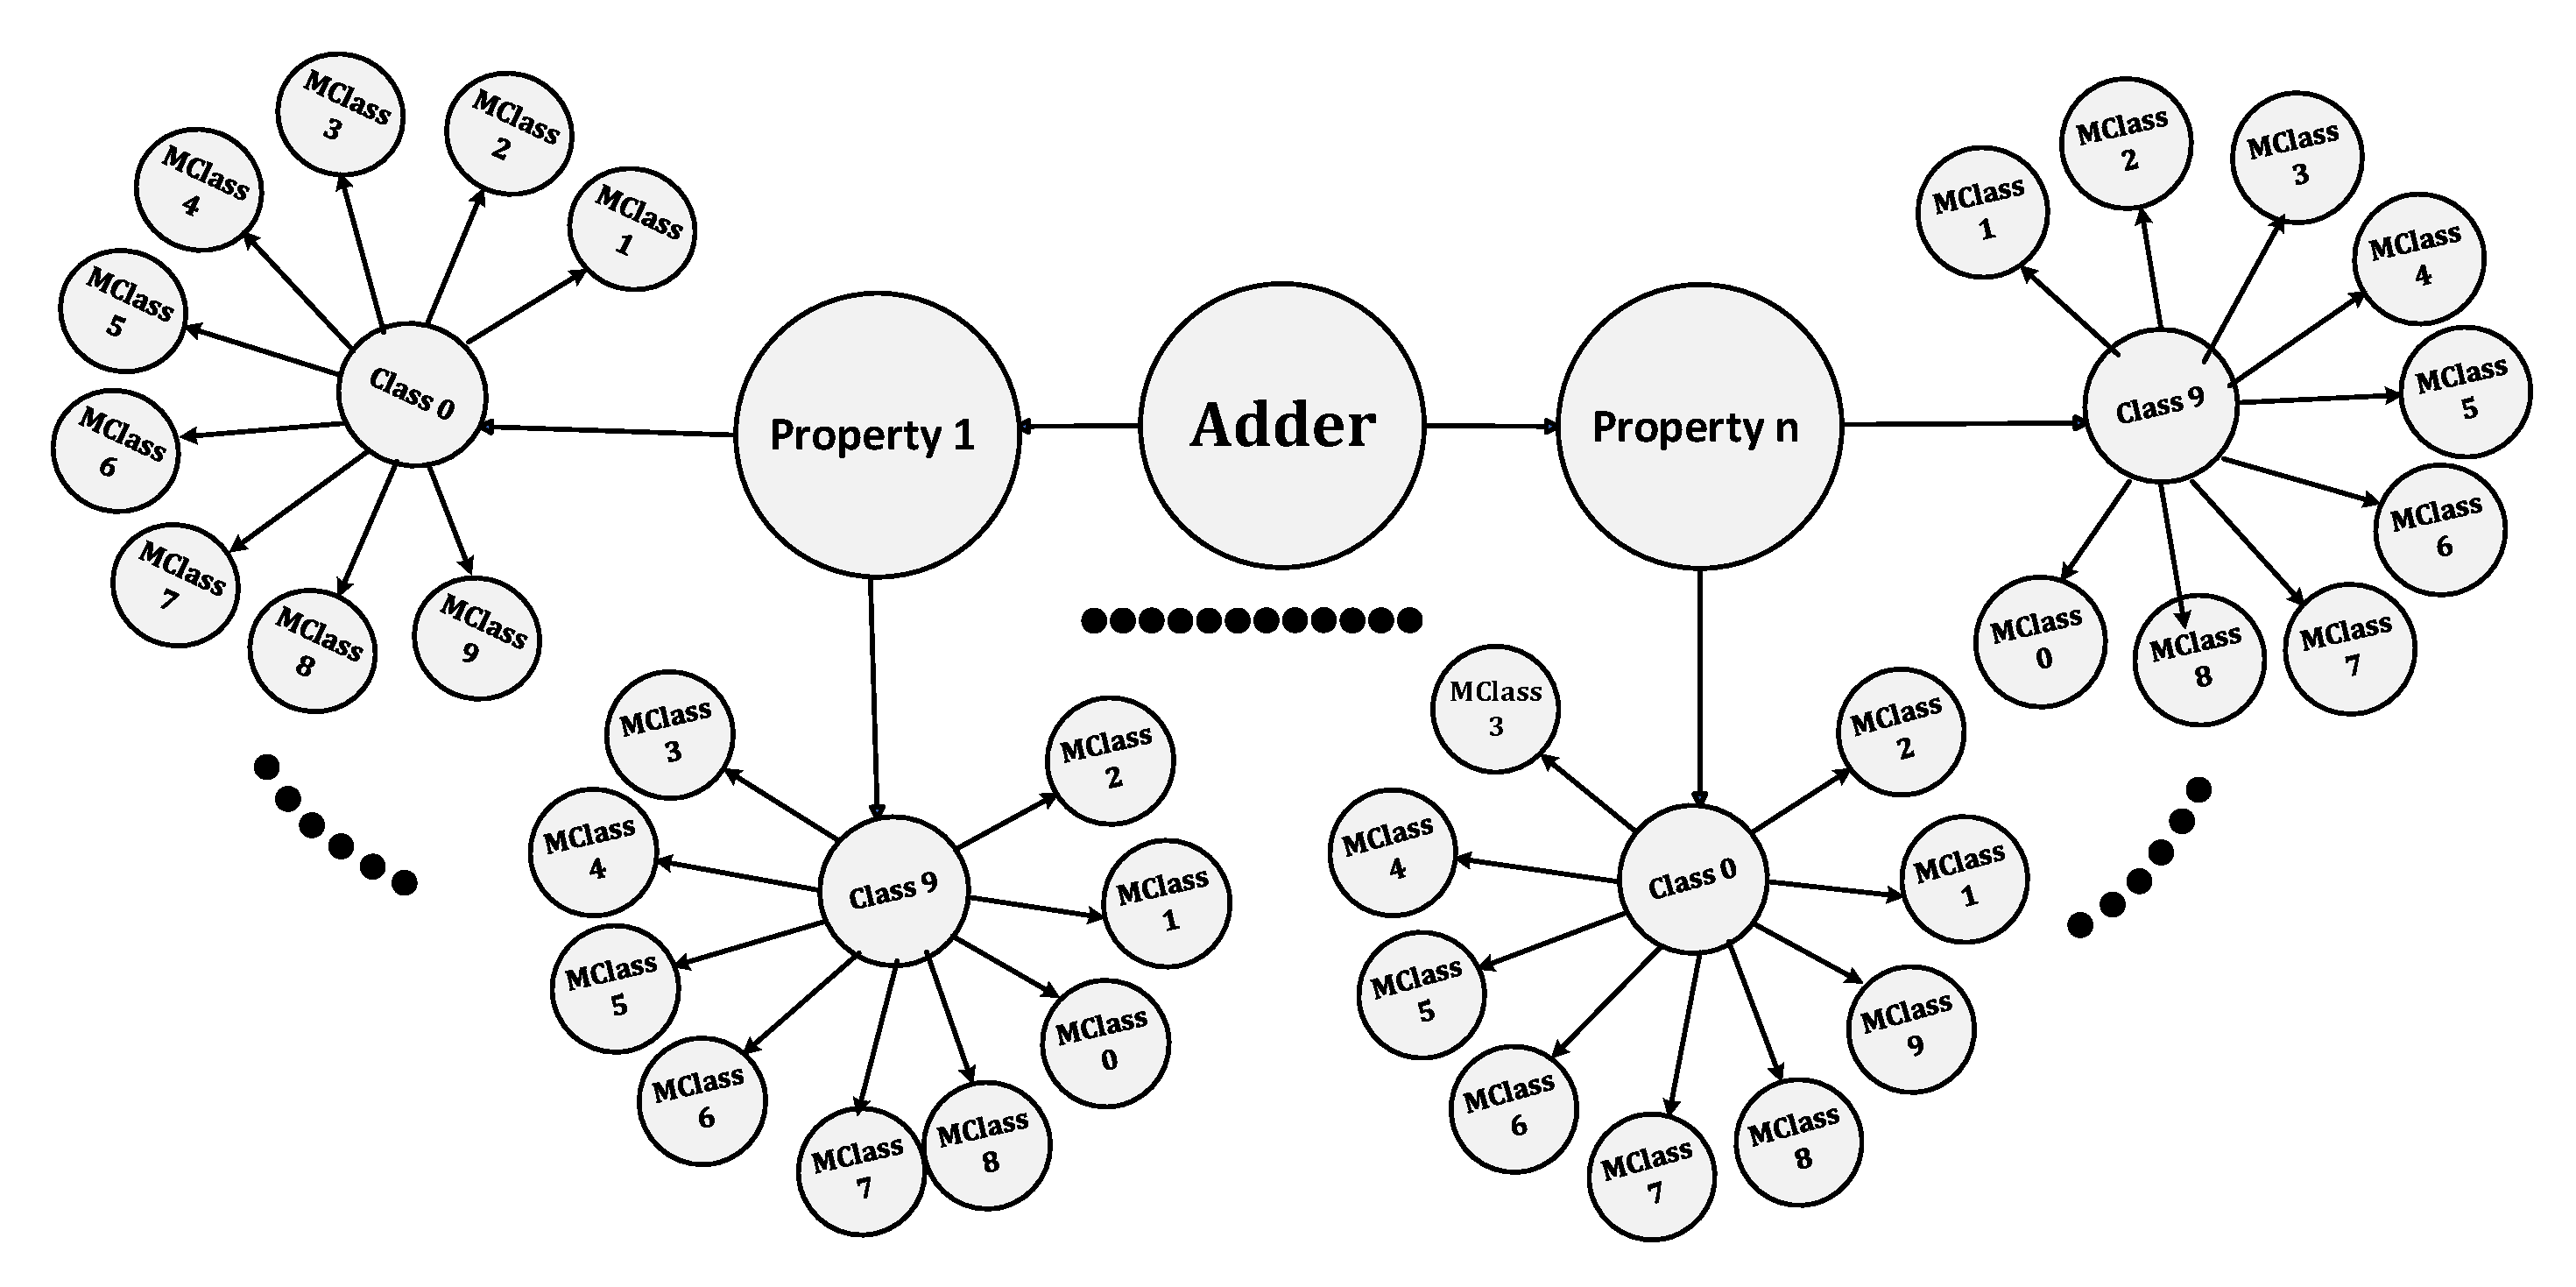
\includegraphics[width=1\textwidth]{figures/step5.pdf}
%     \caption{Error Summarization}
%     \label{Summarization}
% \end{figure*}

% \subsection{Use Cases and Examples}

% To illustrate the application of ProbLog for global robustness in real-world scenarios, we present the following use cases:

% \subsubsection{Use Case 1: Handwritten Digit Recognition}

% \textbf{Scenario:} Consider an AI system designed to recognize handwritten digits, such as the MNIST dataset. The system is evaluated under various transformations, including noise addition, rotation, and brightness adjustment. The goal is to determine the global robustness of the system in recognizing digit pairs correctly under these properties.

% The tables below provide the probabilities for correctly recognizing digit pairs under different conditions (AND and OR relationships) for an MNIST 2-digit addition system. Each world represents a different combination of transformations applied to the digits.

% \begin{table}[h]
%     \centering
%     \caption{Specification Probabilities for MNIST 2-Digit Addition Under Different Transformations}
%     \label{tab:mnist_prob_and_or}
%     \resizebox{\textwidth}{!}{%
%     \begin{tabular}{|c|c|c|c|c|c|}
%     \hline
%     \textbf{World} & \textbf{Conditions} & \textbf{Probability Expression (AND)} & \textbf{Probability (AND)} & \textbf{Probability Expression (OR)} & \textbf{Probability (OR)} \\
%     \hline
%     $w_1$ & \{noise(0), noise(1)\} & $0.85 \cdot 0.8$ & $0.68$ & $0.85 + 0.8 - (0.85 \cdot 0.8)$ & $0.97$ \\
%     $w_2$ & \{noise(0), correct(1)\} & $0.85 \cdot 0.9$ & $0.765$ & $0.85 + 0.9 - (0.85 \cdot 0.9)$ & $0.985$ \\
%     $w_3$ & \{correct(0), noise(1)\} & $0.9 \cdot 0.8$ & $0.72$ & $0.9 + 0.8 - (0.9 \cdot 0.8)$ & $0.98$ \\
%     $w_4$ & \{rotation(0), correct(1)\} & $0.88 \cdot 0.9$ & $0.792$ & $0.88 + 0.9 - (0.88 \cdot 0.9)$ & $0.992$ \\
%     $w_5$ & \{correct(0), rotation(1)\} & $0.9 \cdot 0.77$ & $0.693$ & $0.9 + 0.77 - (0.9 \cdot 0.77)$ & $0.977$ \\
%     $w_6$ & \{rotation(0), rotation(1)\} & $0.88 \cdot 0.77$ & $0.6776$ & $0.88 + 0.77 - (0.88 \cdot 0.77)$ & $0.9696$ \\
%     $w_7$ & \{noise(0), rotation(1)\} & $0.85 \cdot 0.77$ & $0.6545$ & $0.85 + 0.77 - (0.85 \cdot 0.77)$ & $0.9655$ \\
%     $w_8$ & \{rotation(0), noise(1)\} & $0.88 \cdot 0.8$ & $0.704$ & $0.88 + 0.8 - (0.88 \cdot 0.8)$ & $0.976$ \\
%     $w_9$ & \{correct(0), correct(1)\} & $0.9 \cdot 0.9$ & $0.81$ & $0.9 + 0.9 - (0.9 \cdot 0.9)$ & $0.99$ \\
%     \hline
%     \end{tabular}
%     }
% \end{table}

% \textbf{Explanation:} The table shows the global correctness probabilities for pairs of digits under various transformation conditions. Each row represents a different combination of transformations applied to the two digits in the pair:
% - AND Probability: The probability that both digits are correctly recognized under the specified transformations.
% - OR Probability: The probability that at least one of the digits is correctly recognized under the specified transformations.

% For example, in world $w_1$, both digits are subjected to noise, leading to an AND probability of $0.68$ and an OR probability of $0.97$.

% \textbf{Problog Code:}
% \begin{mdframed}[leftline=false, rightline=false, topline=true, bottomline=true]
% \scriptsize
% \begin{verbatim}
% % Define probabilities for digit 0 under different transformations
% 0.9::noise_0. % Digit 0 correctly predicted with 90% probability under noise
% 0.85::brightness_0. % Digit 0 correctly predicted with 85% probability under brightness
% 0.88::rotation_0. % Digit 0 correctly predicted with 88% probability under rotation

% % Define probabilities for digit 1 under different transformations
% 0.8::noise_1. % Digit 1 correctly predicted with 80% probability under noise
% 0.75::brightness_1. % Digit 1 correctly predicted with 75% probability under brightness
% 0.77::rotation_1. % Digit 1 correctly predicted with 77% probability under rotation

% % Define rules for correct prediction under each transformation for digit 0
% correct_noise_0 :- noise_0.
% correct_brightness_0 :- brightness_0.
% correct_rotation_0 :- rotation_0.

% % Define rules for correct prediction under each transformation for digit 1
% correct_noise_1 :- noise_1.
% correct_brightness_1 :- brightness_1.
% correct_rotation_1 :- rotation_1.

% % Define rules for incorrect prediction under each transformation for digit 0
% wrong_noise_0 :- +correct_noise_0.
% wrong_brightness_0 :- +correct_brightness_0.
% wrong_rotation_0 :- +correct_rotation_0.

% % Define rules for incorrect prediction under each transformation for digit 1
% wrong_noise_1 :- +correct_noise_1.
% wrong_brightness_1 :- +correct_brightness_1.
% wrong_rotation_1 :- +correct_rotation_1.

% % Define rules for correct prediction of both digits under noise
% pair_correct_noise_0_1 :- correct_noise_0, correct_noise_1.
% % Define rules for incorrect prediction of both digits under noise
% pair_wrong_noise_0_1 :- wrong_noise_0, wrong_noise_1.

% % Define global correctness based on either both correct or both incorrect under noise
% global_correct_noise_0_1 :- pair_correct_noise_0_1; pair_wrong_noise_0_1.

% % Query the global correctness under noise
% query(global_correct_noise_0_1).
% \end{verbatim}
% \end{mdframed}
% \captionof{figure}{Problog code snippet for evaluating handwritten digit recognition under noise, brightness, and rotation transformations.}

% \textbf{Explanation:} In this scenario, we are interested in the global correctness of recognizing pairs of digits (0 and 1) under different transformations. The ProbLog code models the local robustness probabilities for each transformation and combines them to evaluate the global correctness.

% \subsubsection{Use Case 2: Autonomous Vehicle Perception}

% \textbf{Scenario:} An AI system used in autonomous vehicles must reliably detect objects such as pedestrians and vehicles under various weather conditions (rain, fog, and snow). The goal is to evaluate the system's robustness in identifying these objects correctly under these weather conditions.

% \begin{mdframed}[leftline=false, rightline=false, topline=true, bottomline=true]
%   \scriptsize
%   \begin{verbatim}

% % Probabilities for Vehicle Detection under Different Weather Conditions
% 0.75::rain_vehicle. % Vehicle correctly detected with 75% probability under rain
% 0.55::fog_vehicle. % Vehicle correctly detected with 55% probability under fog
% 0.7::snow_vehicle. % Vehicle correctly detected with 70% probability under snow

% % Correct Detection Rules for Vehicle
% correct_rain_vehicle :- rain_vehicle.
% correct_fog_vehicle :- fog_vehicle.
% correct_snow_vehicle :- snow_vehicle.

% % Incorrect Detection Rules for Vehicle
% wrong_rain_vehicle :- +correct_rain_vehicle.
% wrong_fog_vehicle :- +correct_fog_vehicle.
% wrong_snow_vehicle :- +correct_snow_vehicle.

% % AND conditions for Vehicle Detection under all weather conditions
% global_correct_vehicle_and :- correct_rain_vehicle, correct_fog_vehicle, correct_snow_vehicle.

% % OR conditions for Vehicle Detection under any weather condition
% global_correct_vehicle_or :- correct_rain_vehicle; correct_fog_vehicle; correct_snow_vehicle.

% % Mixed conditions (AND & OR) for Vehicle Detection
% global_correct_mixed_vehicle :- correct_rain_vehicle, (correct_fog_vehicle; correct_snow_vehicle).

% % Queries for Global Correctness
% query(global_correct_vehicle_and).
% query(global_correct_vehicle_or).
% query(global_correct_mixed_vehicle).
% \end{verbatim}
% \end{mdframed}
% \captionof{figure}{Problog code snippet for evaluating vehicle detection under different weather conditions.}

% \textbf{Explanation:} The ProbLog code assesses the global robustness of the AI system in detecting objects (vehicles) under individual and combined weather conditions. This ensures that the system can reliably perform in diverse environmental scenarios.

% \begin{table}[h]
%   \centering
%   \caption{Specification Probabilities (AND) for Vehicle Detection Under Different Weather Conditions \\
%   \( P(A \cap B \cap C) = P(A) \times P(B) \times P(C) \)}
%   \label{tab:veh_prob_and}
%   \resizebox{\textwidth}{!}{%
%   \begin{tabular}{|c|c|c|c|}
%   \hline
%   \textbf{World} & \textbf{Conditions} & \textbf{Probability Expression (AND)} & \textbf{Probability (AND)} \\
%   \hline
%   $w_1$ & \{rain, fog\} & $0.75 \times 0.55$ & $0.4125$ \\
%   $w_2$ & \{rain, snow\} & $0.75 \times 0.7$ & $0.525$ \\
%   $w_3$ & \{rain, sand\} & $0.75 \times 0.6$ & $0.45$ \\
%   $w_4$ & \{fog, snow\} & $0.55 \times 0.7$ & $0.385$ \\
%   $w_5$ & \{fog, sand\} & $0.55 \times 0.6$ & $0.33$ \\
%   $w_6$ & \{snow, sand\} & $0.7 \times 0.6$ & $0.42$ \\
%   $w_7$ & \{rain, fog, snow\} & $0.75 \times 0.55 \times 0.7$ & $0.28875$ \\
%   $w_8$ & \{rain, fog, sand\} & $0.75 \times 0.55 \times 0.6$ & $0.2475$ \\
%   $w_9$ & \{rain, snow, sand\} & $0.75 \times 0.7 \times 0.6$ & $0.315$ \\
%   $w_{10}$ & \{fog, snow, sand\} & $0.55 \times 0.7 \times 0.6$ & $0.231$ \\
%   \hline
%   \end{tabular}
%   }
% \end{table}

% \textbf{Explanation:} This table shows the global correctness probabilities for detecting vehicles under different combinations of weather conditions using AND relationships. Each row represents a different combination of weather conditions applied to the detection scenario:
% - AND Probability: The probability that the vehicle is correctly detected under all specified weather conditions.

% For example, in world $w_1$, the vehicle detection system is subjected to rain and fog, leading to an AND probability of $0.4125$.

% \begin{table}[h]
%   \centering
%   \caption{Specification Probabilities (OR) for Vehicle Detection Under Different Weather Conditions \\
%   \( P(A \cup B \cup C) = P(A) + P(B) + P(C) - P(A \cap B) - P(A \cap C) - P(B \cap C) + P(A \cap B \cap C) \)}
%   \label{tab:veh_prob_or}
%   \resizebox{\textwidth}{!}{%
%   \begin{tabular}{|c|c|c|c|}
%   \hline
%   \textbf{World} & \textbf{Conditions} & \textbf{Probability Expression (OR)} & \textbf{Probability (OR)} \\
%   \hline
%   $w_1$ & \{rain; fog\} & $0.75 + 0.55 - (0.75 \times 0.55)$ & $0.8875$ \\
%   $w_2$ & \{rain; snow\} & $0.75 + 0.7 - (0.75 \times 0.7)$ & $0.925$ \\
%   $w_3$ & \{rain; sand\} & $0.75 + 0.6 - (0.75 \times 0.6)$ & $0.9$ \\
%   $w_4$ & \{fog; snow\} & $0.55 + 0.7 - (0.55 \times 0.7)$ & $0.835$ \\
%   $w_5$ & \{fog; sand\} & $0.55 + 0.6 - (0.55 \times 0.6)$ & $0.82$ \\
%   $w_6$ & \{snow; sand\} & $0.7 + 0.6 - (0.7 \times 0.6)$ & $0.88$ \\
%   $w_7$ & \{rain; fog; snow\} & $0.75 + 0.55 + 0.7 - (0.75 \times 0.55) - (0.75 \times 0.7) - (0.55 \times 0.7) + (0.75 \times 0.55 \times 0.7)$ & $0.966625$ \\
%   $w_8$ & \{rain; fog; sand\} & $0.75 + 0.55 + 0.6 - (0.75 \times 0.55) - (0.75 \times 0.6) - (0.55 \times 0.6) + (0.75 \times 0.55 \times 0.6)$ & $0.95125$ \\
%   $w_9$ & \{rain; snow; sand\} & $0.75 + 0.7 + 0.6 - (0.75 \times 0.7) - (0.75 \times 0.6) - (0.7 \times 0.6) + (0.75 \times 0.7 \times 0.6)$ & $0.967$ \\
%   $w_{10}$ & \{fog; snow; sand\} & $0.55 + 0.7 + 0.6 - (0.55 \times 0.7) - (0.55 \times 0.6) - (0.7 \times 0.6) + (0.55 \times 0.7 \times 0.6)$ & $0.938$ \\
%   \hline
%   \end{tabular}
%   }
% \end{table}

% \textbf{Explanation:} This table shows the global correctness probabilities for detecting vehicles under different combinations of weather conditions using OR relationships. Each row represents a different combination of weather conditions applied to the detection scenario:
% - OR Probability: The probability that the vehicle is correctly detected under at least one of the specified weather conditions.

% For example, in world $w_1$, the vehicle detection system is subjected to rain and fog, leading to an OR probability of $0.8875$.

% \section{Error Summarization}

% Error summarization involves evaluating the performance of the AI system by identifying and quantifying errors. We use Bayesian Network-based Coverage Metrics to assess both local and global coverage. Two testing coverage metrics are defined in Figure~\ref{Coverage}: local coverage (LC) and global coverage (GC).

% \begin{figure*}[h]
%     \centering
%     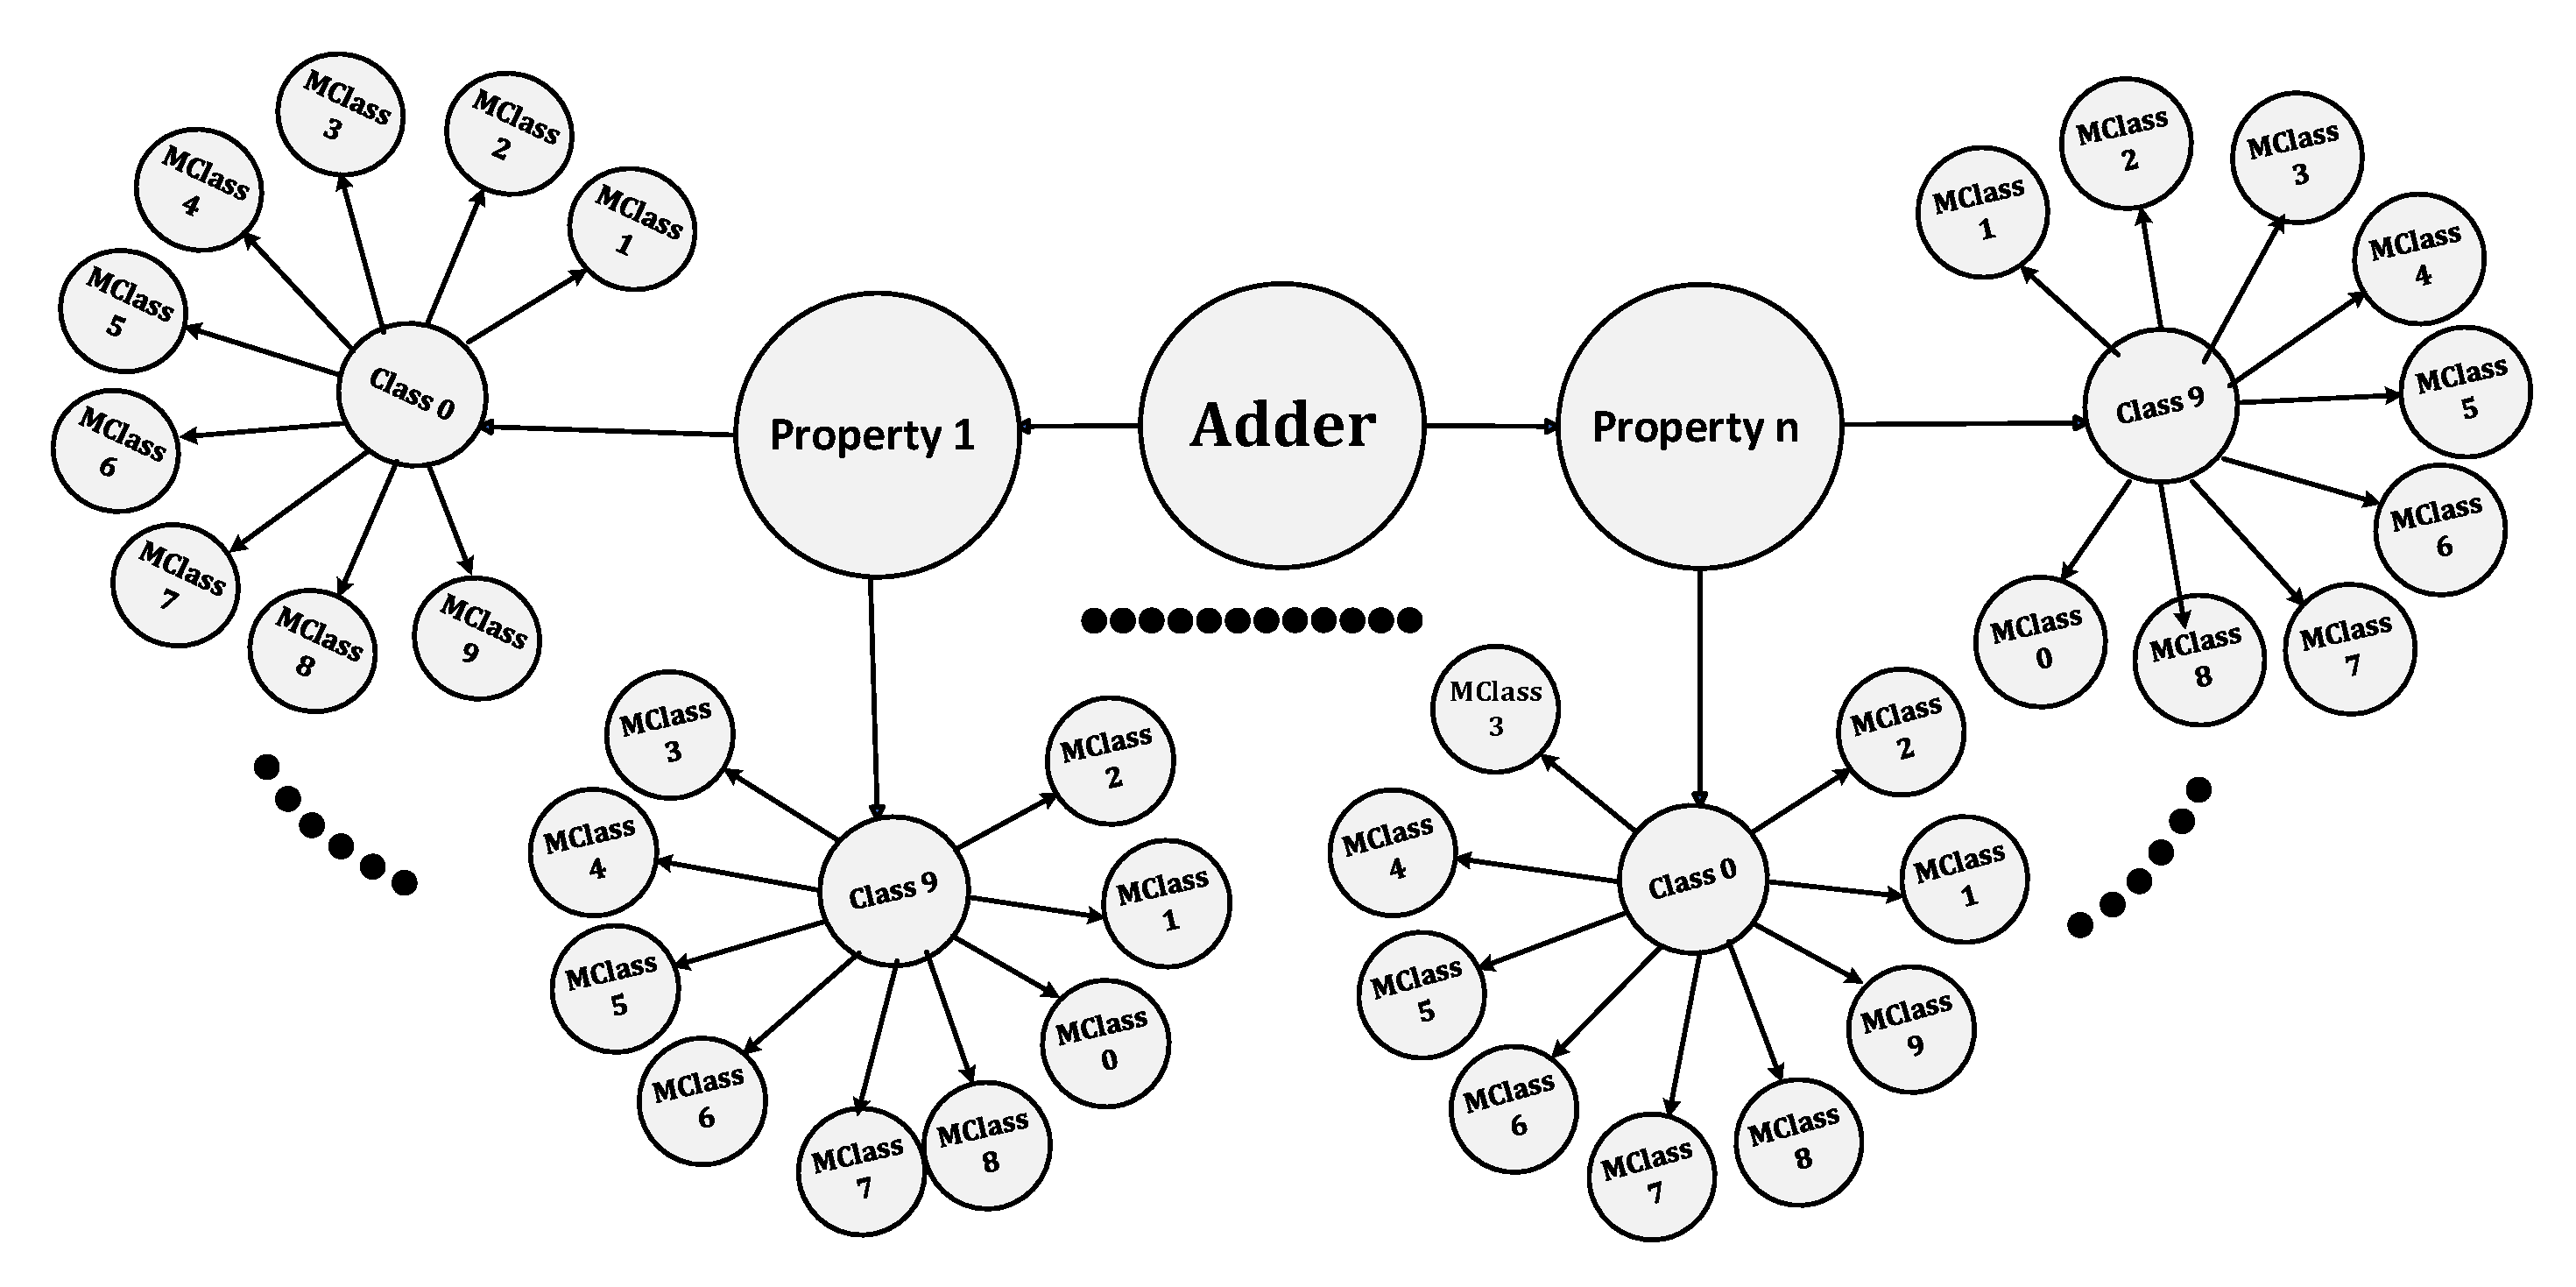
\includegraphics[width=\textwidth]{figures/step5.pdf}
%     \caption{Error Summarization}
%     \label{Summarization}
% \end{figure*}
\section{Error Summarization}

Error summarization involves evaluating the performance of the AI system by identifying and quantifying errors. We use Bayesian Network-based Coverage Metrics to assess both local and global coverage. Two testing coverage metrics are defined in Figure~\ref{Coverage}: local coverage (LC) and global coverage (GC).

\begin{figure*}[h]
    \centering
    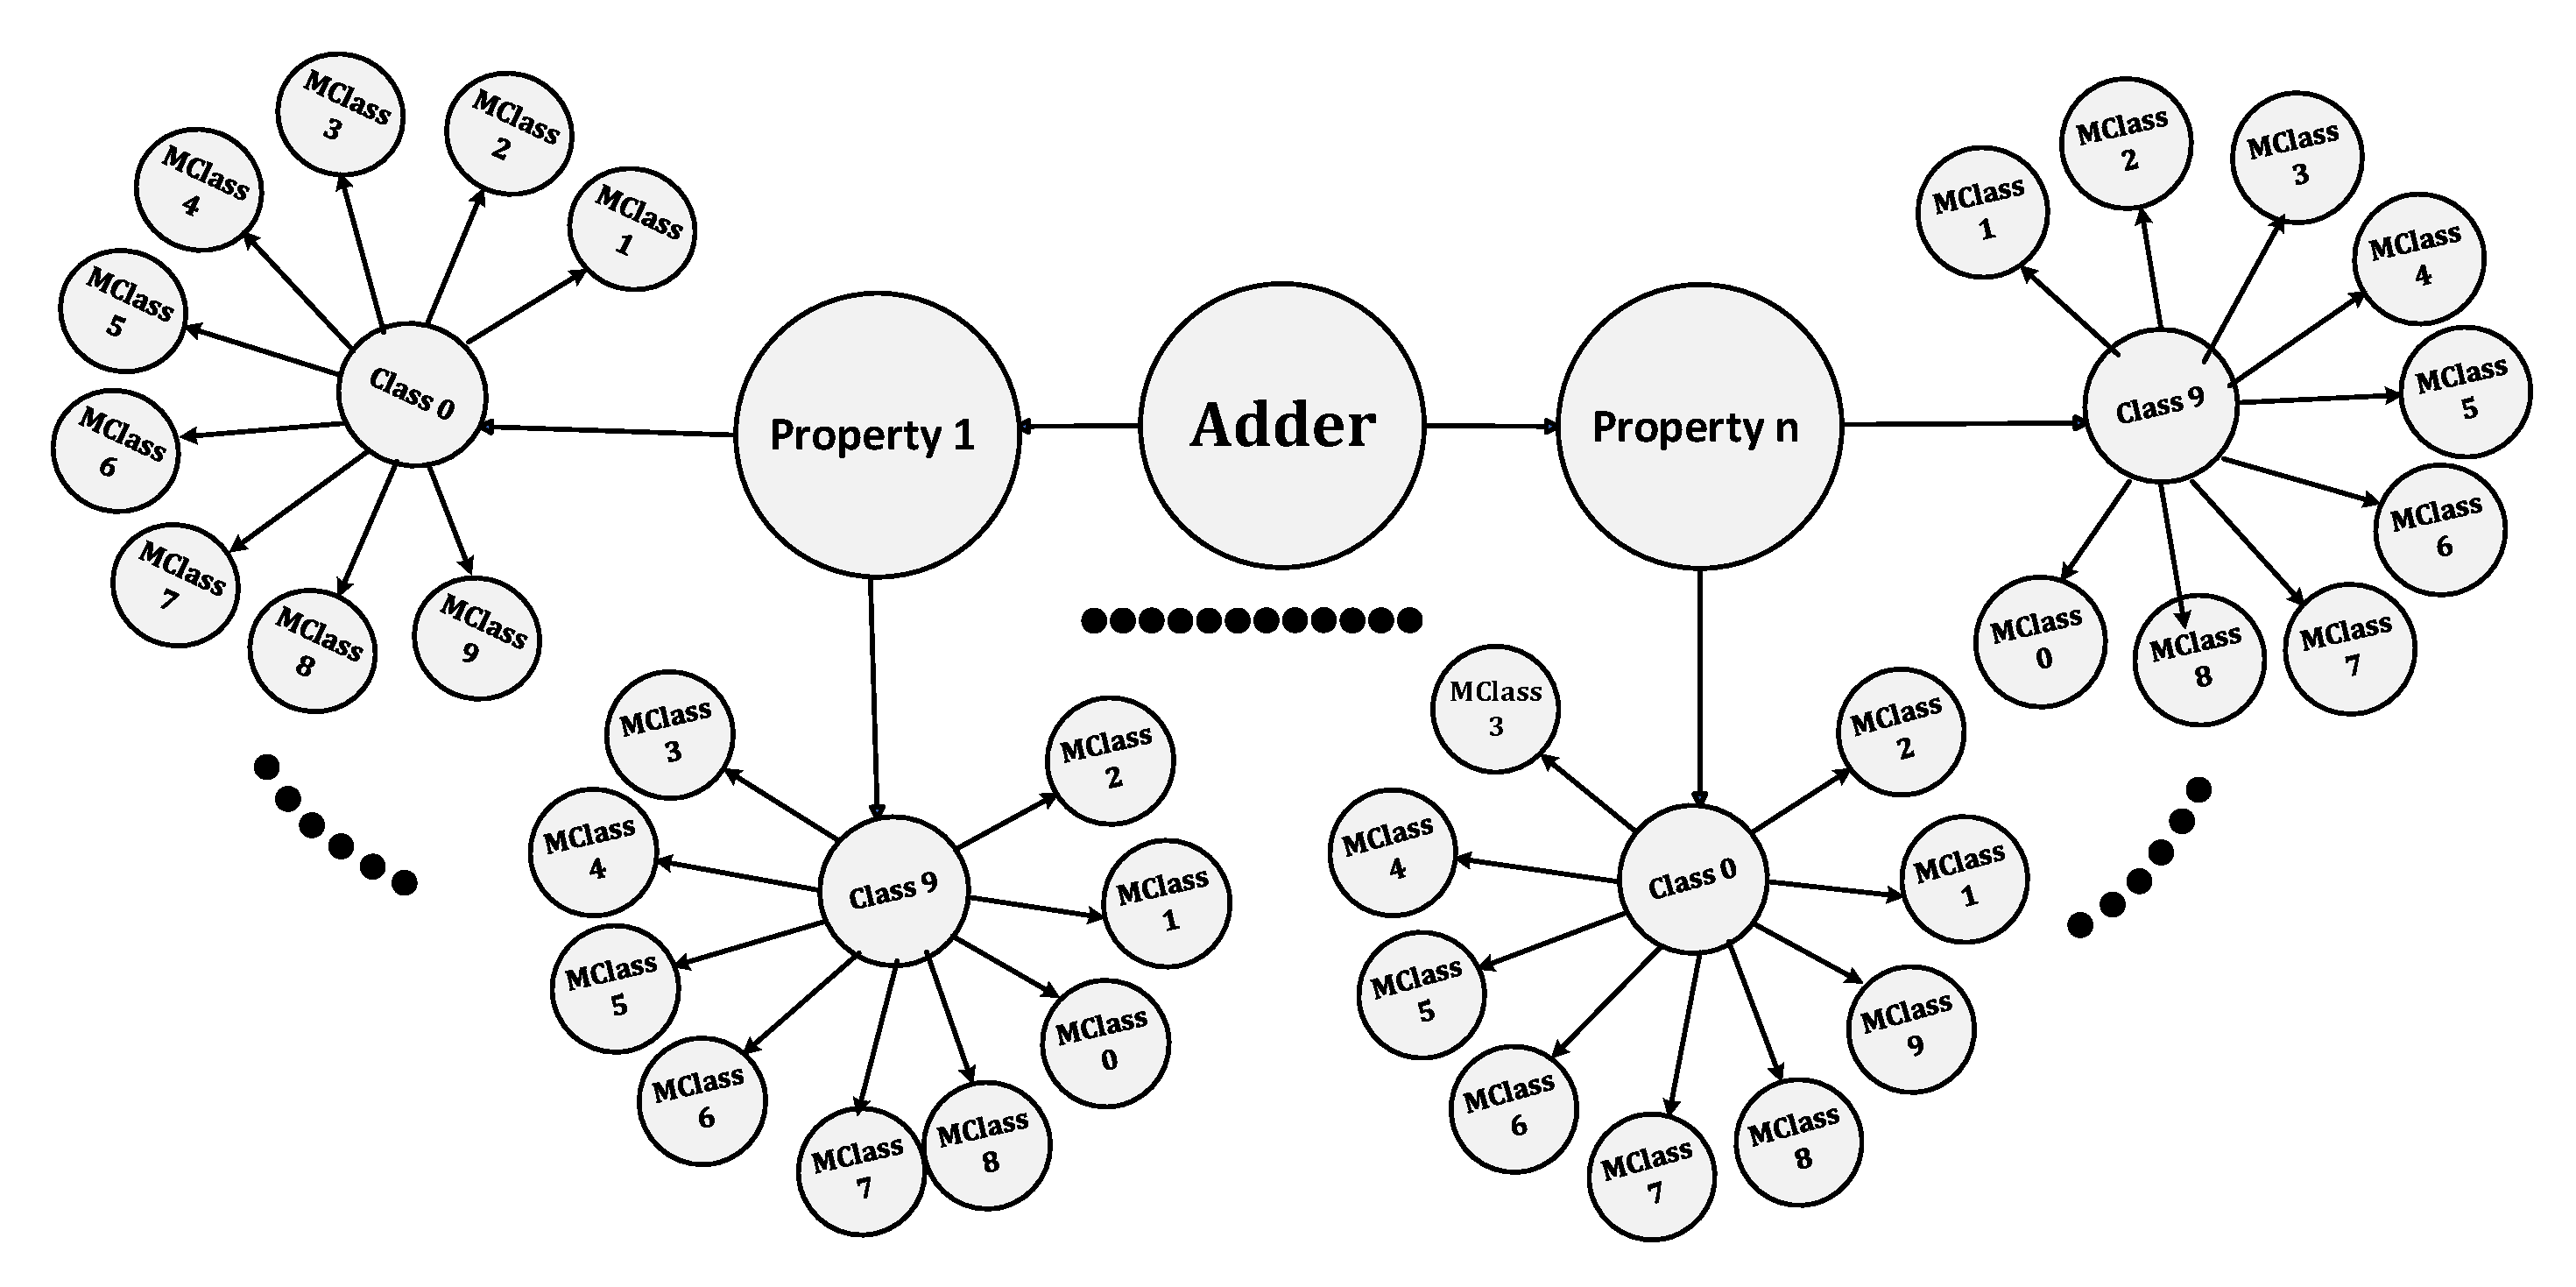
\includegraphics[width=\textwidth]{figures/step5.pdf}
    \caption{Error Summarization}
    \label{Summarization}
\end{figure*}



\section{Algorithm for Evaluating Model Robustness Using ProbLog}

\begin{algorithm}
  \caption{Evaluating Model Robustness Using ProbLog}
  \label{alg:model_robustness}
  \begin{algorithmic}[1]

  \REQUIRE $M$: Pre-trained model
  \REQUIRE $D$: Dataset
  \REQUIRE $N$: Number of samples per class
  \REQUIRE $P$: Set of properties

  \ENSURE $G$: Global correctness values for each specification

  \STATE \textbf{Load and Preprocess Data}
  \STATE $(X_{\text{train}}, y_{\text{train}}), (X_{\text{test}}, y_{\text{test}}) \leftarrow \text{load\_data}(D)$
  \STATE $X_{\text{test}} \leftarrow \text{preprocess\_data}(X_{\text{test}})$
  \STATE $\hat{Y} \leftarrow M.\text{predict}(X_{\text{test}})$
  \STATE $\hat{y} \leftarrow \text{extract\_predictions}(\hat{Y})$

  \STATE \textbf{Determine Number of Classes}
  \STATE $C \leftarrow \text{num\_classes}(y_{\text{test}})$ \COMMENT{Number of unique classes in the dataset}

  \STATE \textbf{Select Correctly Classified Samples}
  \STATE $\text{correct\_samples} \leftarrow \{ \}$
  \FOR{$c = 0$ \TO $C-1$} 
      \STATE $\text{correct\_samples}[c] \leftarrow \text{select\_correct\_samples}(X_{\text{test}}, y_{\text{test}}, \hat{y}, c, N)$
  \ENDFOR

  \STATE \textbf{Define Transformation Functions}
  \STATE $\text{define\_transformations}()$

  \STATE \textbf{Generate Test Cases}
  \FOR{$c = 0$ \TO $C-1$}
      \FORALL{$x \in \text{correct\_samples}[c]$}
          \FORALL{$T \in P$}
              \STATE $\text{generate\_test\_cases}(x, T)$
          \ENDFOR
      \ENDFOR
  \ENDFOR

  \STATE \textbf{Evaluate Model on Transformations}
  \FOR{$c = 0$ \TO $C-1$}
      \FORALL{$\text{property} \in P$}
          \STATE $L_{c, \text{property}} \leftarrow \text{compute\_accuracy}(M, \text{property}, c)$
      \ENDFOR
  \ENDFOR

  \STATE \textbf{Specification Definitions:}
  \STATE Specification1: $P(\text{Property1} \cap \text{Property2}) = P(\text{Property1}) \times P(\text{Property2})$ \COMMENT{AND relationship}
  \STATE Specification2: $P(\text{Property1} \cup \text{Property2}) = P(\text{Property1}) + P(\text{Property2}) - P(\text{Property1} \cap \text{Property2})$ \COMMENT{OR relationship}
  \STATE Specification3: Custom definitions
  \STATE \ldots

  \STATE \textbf{Generate and Evaluate ProbLog Code for Each Specification}
  \STATE Initialize $G$ as an empty list

  \FOR{$\text{spec} = 1$ \TO $\text{num\_specs}$}
      \STATE $\text{ProbLog Code}_{\text{spec}} \leftarrow \text{generate\_problog\_code}(L_{c, \text{property}}, \text{spec})$
      \STATE $G_{\text{spec}} \leftarrow \text{evaluate\_problog}(\text{ProbLog Code}_{\text{spec}})$
      \STATE Append $G_{\text{spec}}$ to $G$
  \ENDFOR

  \RETURN $G$
  \end{algorithmic}
\end{algorithm}

